\documentclass{article}

\date{22 juin 2024}
\usepackage[nb-sem=27, auteurs={Vangilluwen Hugo}]{../kholles}

\begin{document}
\maketitle

\begin{question_kholle}
	[{Soit $f \in \ContM{[a;b]}{}$. \\
				L'ensemble $\{ |f(t)| \;|\; t \in [a;b] \}$ admet une borne supérieur notée $\norminf{f}$.}]
	{Norme uniforme d'une fonction continue par morceaux}

	Montrons que sur chaque morceau, $f$ est bornée.

	Soit $\sigma = (x_i)_{0 \leqslant i \leqslant N} \in \mathcal{S}([a;b])$ adaptée à $f$.
	Soit $i \in \lient 0; N-1 \rient$. Posons $f_i = f_{|]x_i;x_{i+1}[}$.
	$f$ étant continue par morceaux, $\exists (l_i^+, l_{i-1}^-) \in \R^2 : \textlim{x}{x_i^+} f_i(x) = l_i^+ \wedge \textlim{x}{x_{i+1}^-} f_i(x) = l_{i+1}^-$.
	Nous pouvons donc prolonger $f_i$ en $\tilde{f_i}$ par continuité en $x_i$ et en $x_{i+1}$.
	Comme $f \in \Cont{0}{[a;b]}{}$, le théorème de Weierstrass s'applique : $\Im \tilde{f_i}$ est bornée (donc $f_i$ aussi). Ainsi $\norminf{f_i}$ est bien défini.

	\noindent $\{ |f(t)| \;|\; t \in [a;b] \}$ est : \begin{itemize}
		\item une partie de \R
		\item non vide car contenant $|f(x)|$.
		\item majorée par $\max \left( \{\norminf{f_i} | i \in \lient 0; N-1 \rient\} \cup \{\norminf{f_i} | i \in \lient 0; N-1 \rient\} \right)$ (ensemble admettant bien un plus grand élément puisque fini)
	\end{itemize}
	Donc $\norminf{f}$ est bien définie.
	\begin{figure}[H]
		\centering
		\begin{tikzpicture}
			\draw[->] (-0.5, 0) -- (5, 0);
			\draw[->] (0, -0.5) -- (0, 5);
			\draw (4, -0.1) node[anchor=north] {$1$} -- (4, 0.1);
			\draw (2, -0.1) node[anchor=north] {$\nicefrac{1}{2}$} -- (2, 0.1);
			\draw (-0.1, 4) node[anchor=east] {$1$} -- (0.1, 4);

			\draw[red] (0, 0) -- (2, 4) -- (4, 0);
			\filldraw[white, draw=red, densely dotted] (2, 3.95) circle (3pt);
			\filldraw[red] (2, 0) circle (2pt);
		\end{tikzpicture}
		\caption{$\norminf{f}$ peut ne pas être atteinte}
	\end{figure}
\end{question_kholle}

\begin{question_kholle}
	[Soit {$f \in \Cont{0}{[a;b]}{}$}.
		\begin{propositions}
			\item $\forall \varepsilon \in \R_+^*, \
				\exists \chi \in \mathcal{E}({[a;b]}, \R) :
				\norminf{f - \chi} \leqslant \varepsilon$
			\item $\forall \varepsilon \in \R_+^*, \
				\exists (\varphi, \psi) \in \mathcal{E}({[a;b]}, \R)^2 :
				\left\{ \begin{matrix}
					\varphi \leqslant f \leqslant \psi \\
					\norminf{\psi - \varphi} \leqslant \varepsilon
				\end{matrix} \right.$
		\end{propositions}]
	{Lemme d'approximation uniforme d'un fonction continue sur un segment par une fonction en escalier}

	Soit $f \in \Cont{0}{[a;b]}{}$. Soit $\varepsilon \in \R_+^*$ \fq. \\
	$(i)$ D'après le théorème de Heine, $f \in \ContU{[a;b]}{}$. Écrivons la définition de uniformément continue pour $\varepsilon$ :
	\begin{equation*}
		\exists \eta \in \R_ +^* : \ \forall (x, y) \in [a;b]^2, \
		|x - y| \leqslant \eta \implies |f(x) - f(y)| \leqslant \varepsilon
	\end{equation*}

	\begin{figure}[H]
		\centering
		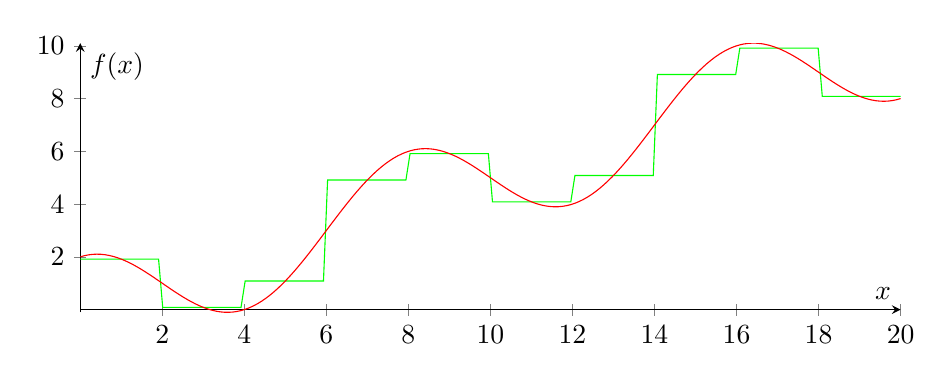
\begin{tikzpicture}
			\begin{axis}[
					axis lines = center,
					xlabel = $x$,
					ylabel = {$f(x)$},
					width=12cm,
					height=5cm
				]
				\addplot[
					domain=0:20,
					samples=200,
					color=green,
				]
				{2*cos((floor(x/2)*2+1)*45) + floor(x/2)+(1/2)};
				\addplot[
					domain=0:20,
					samples=200,
					color=red,
				]
				{2*cos(x*45) + x/2};
			\end{axis}
		\end{tikzpicture}
		\caption{Fonction en escalier "approximant" une fonction continue}
	\end{figure}

	\noindent Cherchons $N$ \tq $\frac{b - a}{N} \leqslant 2 \eta$. C'est-à-dire $N \geqslant \frac{b - a}{2 \eta}$.
	Posons donc $N = \lceil \frac{b - a}{2 \eta} \rceil$ et $\eta' = \frac{b-a}{N}$ de sorte que $\eta' \leqslant 2\eta$.

	Définissons $\chi \in \mathcal{E}({[a;b]}, \R)$ par
	\begin{equation*}
		\chi \left| \begin{array}{ccl}
			[a;b] & \rightarrow & \R                                                                                                                                                     \\
			x     & \mapsto     & \left\{ \begin{array}{ll}
				                              f(x)                                                                                        & \text{ si } \exists n \in \N : \ x = a + n \eta' \\
				                              f\left(a + \eta' \left( \lfloor \frac{x-a}{\eta'} \rfloor + \nicefrac{1}{2} \right) \right) & \text{ sinon }
			                              \end{array} \right.
		\end{array} \right.
	\end{equation*}
	Ceci est bien une fonction en escalier car $(a + k \eta')_{0 \leqslant k \leqslant N}$ est une subdivision adaptée. En effet, $\forall k \in \lient 0; N-1 \rient, \ f_{|]a+k\eta';a+(k+1)\eta'[} =f\left( a + \eta' \left( \lfloor \frac{x-a}{\eta'} \rfloor + \nicefrac{1}{2} \right) \right) \cdot \widetilde{1}_{]a+k\eta';a=(k+1)\eta'[}$.

	Soit $x \in [a; b]$.
	Si $\exists n \in \N : \ x = a + n \eta'$ alors $|f(x) - \chi(x)| = 0$.
	Sinon $0 \leqslant \frac{x - a} {\eta'} - \lfloor \frac{x-a}{\eta'} \rfloor \leqslant 1$.
	D'où $0 \leqslant (x - a) - \eta' \lfloor \frac{x-a}{\eta'} \rfloor \leqslant \eta'$.
	Donc, en enlevant $\nicefrac{\eta'}{2}$, $- \frac{\eta'}{2} \leqslant a + \eta' \left( \lfloor \frac{x-a}{2 \eta} \rfloor + \nicefrac{1}{2} \right) \leqslant \frac{\eta'}{2}$.
	Par définition de $\eta'$, \ $- \eta \leqslant a + \eta' \left( \lfloor \frac{x-a}{2 \eta} \rfloor + \nicefrac{1}{2} \right) \leqslant \eta$.
	Par définition de $\eta$, on a $|f(x) - f\left(a + 2 \eta \left( \lfloor \frac{x-a}{2 \eta} \rfloor + \nicefrac{1}{2} \right) \right)| \leqslant \varepsilon$.

	Ainsi, nous avons bien $\norminf{f - \chi} \leqslant \varepsilon$.
	\bigbreak

	$(ii)$ Écrivons la définition de uniformément continue pour $\varepsilon$ :
	\begin{equation*}
		\exists \eta \in \R_ +^* : \ \forall (x, y) \in [a;b]^2, \
		|x - y| \leqslant \eta \implies |f(x) - f(y)| \leqslant \varepsilon
	\end{equation*}
	Définissons $\varphi \in \mathcal{E}({[a;b]}, \R)$ par
	\begin{equation*}
		\left| \begin{matrix}
			[a;b] & \rightarrow & \R                                                                                                                                                                                                \\
			x     & \mapsto     & \left\{ \begin{matrix}
				                              f(x)                                                                                                                                    & \text{ si } \exists n \in \N : \ x = a + n \eta \\
				                              \inf f\left( \; ]a + \eta \lfloor \frac{x-a}{\eta'} \rfloor; a + \eta \left( \lfloor \frac{x-a}{\eta'} \rfloor + 1 \right) [ \; \right) & \text{ sinon }
			                              \end{matrix} \right.
		\end{matrix} \right.
	\end{equation*}
	Définissons $\psi \in \mathcal{E}({[a;b]}, \R)$ par
	\begin{equation*}
		\left| \begin{matrix}
			[a;b] & \rightarrow & \R                                                                                                                                                                                               \\
			x     & \mapsto     & \left\{ \begin{matrix}
				                              f(x)                                                                                                                                   & \text{ si } \exists n \in \N : \ x = a + n \eta \\
				                              \sup f\left( \; ] a + \eta \lfloor \frac{x-a}{\eta'} \rfloor; a + \eta \left( \lfloor \frac{x-a}{\eta'} \rfloor + 1\right)[ \; \right) & \text{ sinon }
			                              \end{matrix} \right.
		\end{matrix} \right.
	\end{equation*}
	Ces deux fonctions sont bien définies car $f_{|] a + \eta \lfloor \frac{x-a}{\eta'} \rfloor; a + \eta \left( \lfloor \frac{x-a}{\eta'} \rfloor + 1\right)[}$ est continue donc, d'après le théorème de Weiertraß, son image admet une borne inférieure et une borne supérieure.
	Elle sont bien en escalier.

	Par définition des bornes inférieures et supérieures, nous avons $\varphi \leqslant f \leqslant \psi$.
	De plus, pour $x \in [a;b]$ \fq, $f_{|] a + \eta \lfloor \frac{x-a}{\eta'} \rfloor; a + \eta \left( \lfloor \frac{x-a}{\eta'} \rfloor + 1\right)[}$ se prolonge par continuité et, d'après le théorème de Weiertraß, atteint ses bornes. Notons $f_i$ et $f_s$ les antécédents respectifs des bornes.
			$(f_i, f_s) \in ] a + \eta \lfloor \frac{x-a}{\eta'} \rfloor; a + \eta \left( \lfloor \frac{x-a}{\eta'} \rfloor + 1\right)[ ^2$ donc $\left|f_i - f_s\right| \leqslant \eta$.
	D'où $\left| f(f_i) - f(f_s) \right| \leqslant \varepsilon$.

	Ainsi, nous avons bien $\norminf{\psi - \varphi} \leqslant \varepsilon$.
\end{question_kholle}
\begin{question_kholle}[{Soit $f \in \mathcal{CM}([a, b], \mathbb{R})$
				Posons

				\begin{align*}
					\mathcal{E}^{-}(f)=\{ \varphi \in \mathcal{E}([a, b],\mathbb{R}) \mid \varphi \leqslant f \} &
					                                                                                             & \mathcal{E}^{+}(f)=\{ \varphi \in \mathcal{E}([a, b],\mathbb{R}) \mid \varphi \geqslant f \}
				\end{align*}

				et

				\begin{align*}
					I^{-}(f)= \left\{ \int_{a}^{b} \varphi(u) \, \mathrm du \Bigg| \varphi \in \mathcal{E}^{-}(f)  \right\}
					 &  &
					I^{+}(f)= \left\{ \int_{a}^{b} \varphi(u) \, \mathrm du \Bigg| \varphi \in \mathcal{E}^{+}(f)  \right\}
				\end{align*}

				Alors $\sup I^{-}(f) = \inf I^{+}(f)$ que l'on notera $\int_{a}^{b} f(u) \, \mathrm du$}]{Définition de l'intégrale de Darboux}

	\begin{itemize}[label=$\lozenge$]
		\item Bonne définition des objets
		      \begin{itemize}[label=$\star$]
			      \item $I^{-}(f)$ est une partie de $\mathbb{R}$
			      \item Non vide car:
			            $$
				            \forall x \in [a, b], f(x) \geqslant - \|f\|_{\infty, [a, b]} \implies \left( \int_{a}^{b} - \|f\|_{\infty,[a, b]} \, \mathrm dt  \right)  \in I^{-}(f)
			            $$
			      \item majorée: soit $\varphi \in \mathcal{E}^{-}(f)$ fixé quelconque.

			            \begin{align*}
				            \forall x \in [a, b], \varphi(x)\leqslant f(x) & \leqslant \|f\|_{\infty, [a, b]}                              \\
				            \implies \varphi                               & \leqslant \|f\|_{\infty[a, b]}                                \\
				            \implies \int_{a}^{b} \varphi(u) \, \mathrm du & \leqslant  \int_{a}^{b} \|f\|_{\infty, [a, b]}  \, \mathrm dt
			            \end{align*}
		      \end{itemize}

		      On procède de la même manière pour la borne inf de $I^{+}(f)$

		\item De plus, $\sup I^{-}(f) \leqslant \inf I^{+}(f)$

		      Soient $(\varphi, \psi) \in \mathcal{E}^{-}(f)\times \mathcal{E}^{+}(f)$ fixés quelconques


		      \begin{align*}
			       & \forall x \in [a, b], \varphi(x) \leqslant f(x) \leqslant \psi(x)                                                                                                           \\
			       & \implies \forall \varphi \in \mathcal{E}^{-}(f), \varphi \leqslant \psi                                & \implies \psi \text{ majore } \mathcal{E}^{-}(f)                   \\
			       &                                                                                                        & \implies \int_{a}^{b} \psi(u) \, \mathrm du  \text{ majore } I^{-} \\
			       & \implies \sup I^{-} \leqslant \int_{a}^{b} \psi(u) \, \mathrm du                                                                                                            \\
			       & \implies \forall \psi \in \mathcal{E}^{+}(f), \sup I^{-} \leqslant \int_{a}^{b} \psi(u)  \, \mathrm du & \implies \sup I^{-} \text{ minore } I^{-}                          \\
			       &                                                                                                        & \implies \sup I^{-} \leqslant \inf I^{+}
		      \end{align*}


		\item Soit $\varepsilon > 0$ fixé quelconque.
		      Appliquons le lemme d'approximation uniforme d'une fonction continue par morceaux par une fonction en escalier pour $\varepsilon \leftarrow \frac{\varepsilon}{b-a}$ quelconque:

		      $$
			      \exists (\varphi, \psi) \in \mathcal{E}([a, b], \mathbb{R})^{2} : \left\{ \begin{array}{ll}
				      \varphi \leqslant f \leqslant \psi \\
				      \|\varphi - \psi\| _{\infty, [a, b]} \leqslant \frac{\varepsilon}{b-a}
			      \end{array}\right.
		      $$

		      Cela implique nécessairement que $\varphi \in \mathcal{E}^{-}(f)$ et $\psi \in \mathcal{E}^{+}(f)$.

		      $$
			      \left\{ \begin{array}{ll}
				      \varphi \in \mathcal{E}^{-}(f) \\
				      \psi \in \mathcal{E}^{+}(f)
			      \end{array}\right. \implies \left\{ \begin{array}{ll}
				      \int_{a}^{b} \varphi (u) \, \mathrm du \leqslant \sup I^{-} \\
				      \int_{a}^{b} \psi(u) \, \mathrm du \geqslant \inf I^{+}
			      \end{array}\right.
		      $$

		      Donc

		      \begin{align*}
			      \int_{a}^{b} \varphi(u) \, \mathrm du  \leqslant \sup I^{-} \leqslant \inf I^{+} \leqslant \int_{a}^{b} \psi(u) \, \mathrm du     \\
			      \implies 0 \leqslant \inf I^{+} - \sup I^{-} \leqslant \int_{a}^{b} \psi(u) \, \mathrm du - \int_{a}^{b} \varphi(u) \, \mathrm du \\
			      \implies 0 \leqslant \inf I^{+} - \sup I^{-} \leqslant \int_{a}^{b} \psi(u) - \varphi(u) \, \mathrm du                            \\
			      \implies 0 \leqslant \inf I^{+} - \sup I^{-} \leqslant \int_{a}^{b} \frac{\varepsilon}{b-a} \, \mathrm du                         \\
			      \implies 0 \leqslant \inf I^{+} - \sup I^{-} \leqslant \frac{(b-a)\varepsilon}{b-a} = \varepsilon
		      \end{align*}


		      Donc en passant à la limite, on retrouve $\inf I^{+} - \sup I^{+} = 0$, d'où l'égalité attendue.
	\end{itemize}
\end{question_kholle}
\begin{question_kholle}{Montrer qu'une fonction positive ou nulle, continue sur un segment et d'intégrale nulle sur ce segment est identique- ment nulle sur ce segment}
	Par l'absurde supposons qu'il existe $f \in \mathcal{C}^{0}([a, b], \mathbb{R})$ telle que $\int_{a}^{b} f(u) \, \mathrm du = 0$ et $f \geqslant 0$ sur $[a, b]$ et $f \neq \tilde{0}$
	Alors $\exists x_{0} \in [a, b]: f(x_{0}) \neq 0 \implies f(x_{0})>0$
	Appliquons la définition de la continuité de $f$ en $x_{0}$ pour $\varepsilon \leftarrow \frac{f(x_{0})}{2}$
	$$
		\exists \eta >0 : \forall x \in [a, b] \cap [x_{0}-\eta, x_{0}+\eta], \lvert f(x)-f(x_{0}) \rvert \leqslant \frac{f(x_{0})}{2}
	$$
	donc
	$$
		\forall x \in [a, b] \cap [x_{0}-\eta, x_{0}+\eta], f(x) \geqslant \frac{f(x_{0})}{2}>0
	$$

	\begin{itemize}
		\item Ainsi, si $x_{0} \in ]a, b[$

		      \begin{align*}
			      \int_{a}^{b} f(u) \, \mathrm du & =  \underbrace{ \int_{a}^{x_{0}-\eta} f(u) \, \mathrm du }_{ \geqslant 0 } + \int_{x_{0}-\eta}^{x_{0}+\eta} f(u) \, \mathrm du + \underbrace{ \int_{x_{0}+\eta}^{b} f(u) \, \mathrm du }_{ \geqslant 0 } \\
			                                      & \geqslant \int_{x_{0}-\eta}^{x_{0}+\eta}f(u)  \, \mathrm du \geqslant \int_{x_{0}-\eta}^{x_{0}+\eta} \frac{f(x_{0})}{2}  \, \mathrm du \geqslant 2 \eta \frac{f(x_{0})}{2} \geqslant \eta f(x_{0}) > 0
		      \end{align*}


		\item Si $x_{0} \in \{ a, b \}$ on effectue le même raisonnement
		      $$
			      \int_{a}^{a+\eta} f(u) \, \mathrm du \geqslant \frac{\eta f(x_{0})}{2} > 0
		      $$
	\end{itemize}
\end{question_kholle}
\begin{question_kholle}{Inégalité de Cauchy Schwartz pour les fonctions continues par morceaux}
	Soient $(f, g) \in \mathcal{CM}([a, b], \mathbb{R})^{2}$
	Posons
	$$
		\forall t \in \mathbb{R}, P(t) = \int_{a}^{b} (f+tg)^{2}(u) \, \mathrm du
	$$
	\begin{align*}
		P(t) = \int_{a}^{b} (f(u)+t\times g(u))^{2} \, \mathrm du & =
		\int_{a}^{b} f(u)^{2} + 2tg(u)f(u)+ t^{2} g(u)^{2} \, \mathrm du                                                                                                                      \\
		                                                          & = \int_{a}^{b} f(u)^{2} \, \mathrm du + 2t\int_{a}^{b} f(u)g(u) \, \mathrm du + t^{2} \int_{a}^{b} g(u)^{2} \, \mathrm du
	\end{align*}
	\begin{itemize}[label=$\lozenge$]
		\item Si $\int_{a}^{b} g(u)^{2} \, \mathrm du = 0$, $P$ est un polynôme affine de signe positif (intégrale d'une fonction positive) donc sa pente est nulle, donc $\int_{a}^{b} f(u)g(u) \, \mathrm du =0$ donc l'inégalité de cauchy schwartz est vraie

		\item Sinon $P$ est un polynôme de degré $2$, positif ou nul, donc le discriminant $\Delta \leqslant 0$ et $\int_{a}^{b} g(u)^{2} \, \mathrm du \geqslant 0$
		      donc
		      $$
			      4\left( \int_{a}^{b} g(u)f(u) \, \mathrm du  \right)^{2} - 4 \int_{a}^{b} f^{2}(u) \, \mathrm du \int_{a}^{b} g^{2}(u) \, \mathrm du \leqslant 0
		      $$
		      Ce qui prouve l'égalité attendue.
	\end{itemize}
	\begin{itemize}[label=$\lozenge$]
		\item Supposons qu'il y a égalité dans l'inégalité de Cauchy-Schwartz, alors
		      \begin{itemize}
			      \item Si $\int_{a}^{b} g^{2}(u) \, \mathrm du \neq 0$
			            $$
				            \Delta = 4\left( \int_{a}^{b} g(u)f(u) \, \mathrm du  \right)^{2} - 4 \int_{a}^{b} f^{2}(u) \, \mathrm du \int_{a}^{b} g^{2}(u) \, \mathrm du =0
			            $$
			            Donc $P$ est un polynôme de degré 2 de discriminant nul : il admet une racine double $t_{0}$
			            Ainsi,
			            $$
				            P(t_{0}) = 0 \implies \int_{a}^{b} (f+t_{0}g)^{2}(u) \, \mathrm du = 0
			            $$
			            Mais, $(f+t_{0}g)^{2}$ est une fonction positive, et continue sur $[a, b]$, donc elle est nulle sur $[a, b]$.
			            Donc $f+t_{0}g = \tilde{0}$ dong $(f, g)$ est liée.

			      \item Sinon, si $\int_{a}^{b} g^{2}(u) \, \mathrm du = 0$, en remarquant que $g^{2}\geqslant 0$ sur $[a, b]$ et que $g^{2}$ est continue, on retrouve que $g = \tilde{0}$ et donc que $(f, g)$ est liée
		      \end{itemize}
		\item Un calcul simple montre que s'il existe une relation de liaison entre deux fonctions continues par morceaux, il y a égalité dans l'inégalité.
	\end{itemize}
\end{question_kholle}
\begin{question_kholle}{Théorème de convergence des sommes de Riemann}
	$f \in \mathcal{C}^{0}([a, b], \mathbb{C}) a\leqslant b$
	En notant $S(f, \sigma, \pi)$ la somme de Riemann de $f$ pour la subdivision pointée $(\sigma, \pi)$.
	$$
		\forall \varepsilon >0, \exists \eta >0: \forall \left\{ \begin{array}{ll}
			\sigma = (x_{i})_{0 \leqslant i \leqslant N} \in \mathcal{S}([a, b]) \\
			\pi = (x_{i}')_{0\leqslant i\leqslant N-1} : x_{i}' \in [x_{i}, x_{i+1 }]
		\end{array}\right. , \delta(\sigma) \leqslant \eta \implies \left\lvert  S(f, \sigma, \pi) - \int_{a}^{b} f(u) \, \mathrm du   \right\rvert \leqslant \varepsilon
	$$

	Soit $\sigma = (x_{j})_{0\leqslant j \leqslant N} \in \mathcal{S}([a, b])$ et $\pi = (x_{i}')_{0 \leqslant i \leqslant N - 1}$ une famille vérifiant $\forall i \in [ \! [ 0, N-1 ] \!], x_{i}' \in [x_{i}, x_{i+1}]$


	\begin{align*}
		\left\lvert  S(f, \sigma, \pi) - \int_{a}^{b} f(t) \, \mathrm dt   \right\rvert & = \left\lvert  \sum_{i=0}^{N-1}f(x_{i}')(x_{i+1}-x_{i}) - \sum_{i=0}^{N - 1}\int_{x_{i}}^{x_{i+1}} f(t) \, \mathrm dt   \right\rvert \\
		                                                                                & = \left\lvert  \sum_{i=0}^{N-1}\int_{x_{i}}^{x_{i+1}} (f(x_{i}')-f(t)) \, \mathrm dt   \right\rvert                                  \\
		                                                                                & \leqslant \sum_{i=0}^{N-1}\left\lvert  \int_{x_{i}}^{x_{i+1}} (f(x_{i}')-f(t)) \, \mathrm dt   \right\rvert                          \\
		                                                                                & \leqslant \sum_{i=0}^{N-1}\int_{x_{i}}^{x_{i+1}} \lvert f(x_{i}') - f(t) \rvert \, \mathrm dt
	\end{align*}


	Soit $\varepsilon > 0$ fixé quelconque, appliquons la continuité uniforme de $f$ pour $\varepsilon \leftarrow \frac{\varepsilon}{b-a}$
	$$
		\exists \eta >0: \forall(x, y) \in [a, b], \lvert x-y \rvert \leqslant \eta \implies \lvert f(x)-f(y) \rvert \leqslant \frac{\varepsilon}{b-a}
	$$
	Fixons un tel $\eta$. Soit $(\sigma, \pi)$ une subdivision pointée de $[a, b]$ fixée quelconque telle que $\delta(\sigma) \leqslant \eta$.
	Soit $i \in [ \! [ 0, N-1 ] \!]$ fixé quelconque.
	$$
		\forall t \in [x_{i}, x_{i+1}], \lvert x_{i}' - t \rvert  \underbrace{ \leqslant }_{ x_{i}\leqslant x_{i}' \leqslant x_{i+1} } \lvert x_{i}-x_{i+1} \rvert \leqslant \delta(\sigma) \leqslant \eta \implies \lvert f(x_{i}') - f(t) \rvert \leqslant \frac{\varepsilon}{b-a}
	$$
	donc,
	$$
		\int_{x_{i}}^{x_{i+1}} \lvert f(x_{i}')-f(t) \rvert  \, \mathrm dt \leqslant \int_{x_{i}}^{x_{i+1}} \frac{\varepsilon}{b-a} \, \mathrm dt = \frac{\varepsilon}{b-a}(x_{i+1}-x_{i})
	$$
	donc
	$$
		\left\lvert  S(f, \sigma, \pi) - \int_{a}^{b} f(t) \, \mathrm dt   \right\rvert \leqslant \sum_{i=0}^{N-1} \int_{x_{i}}^{x_{i+1}} \lvert f(x_{i}')-f(t) \rvert  \, \mathrm dt \leqslant \sum_{i=0}^{N-1} \frac{\varepsilon}{b-a}(x_{i+1}-x_{i})  = \frac{\varepsilon}{b-a} \underbrace{ \sum_{i=0}^{N-1}(x_{i+1}-x_{i}) }_{ b-a } = \varepsilon
	$$
	donc
	$$
		\left\lvert  S(f, \sigma, \pi) - \int_{a}^{b} f(t) \, \mathrm dt   \right\rvert  \leqslant \varepsilon
	$$
\end{question_kholle}

\begin{question_kholle}{Inégalité triangulaire pour les fonctions continues par morceaux à valeurs complexes}

	Soit $f \in \mathcal{CM}([a, b], \mathbb{C})$ cela implique donc que $\lvert f \rvert \in \mathcal{CM}([a, b], \mathbb{C})$
	D'après le lemme d'approximation uniforme d'une fonction par une fonction uniforme
	$$
		\exists (\chi_{k})_{k \in \mathbb{N}} \in (\mathcal{E}([a, b], \mathbb{R}))^{\mathbb{N}} : \left\{ \begin{array}{ll}
			\forall k \in \mathbb{N}, \|f-\chi_{k}\|_{\infty, [a, b]} \leqslant \frac{1}{2^{k}} \\
			\int_{a}^{b} \chi_{k}(u) \, \mathrm du \xrightarrow[k \to \infty]{} \int_{a}^{b} f(u) \, \mathrm du
		\end{array}\right.
	$$

	$$
		\forall k \in \mathbb{N}, \forall x \in [a, b], \lvert \lvert \chi_{k}(x) \rvert - \lvert f(x) \rvert  \rvert \leqslant \lvert f(x) - \chi_{k}(x) \rvert \leqslant \frac{1}{2^{k}}
	$$
	donc
	$$
		\|\lvert f \rvert - \lvert \chi_{k} \rvert \|_{\infty}\leqslant \frac{1}{2^{k}} \implies \int_{a}^{b} \lvert \chi_{k} \rvert (u) \, \mathrm du \xrightarrow[k \to \infty]{} \int_{a}^{b} \lvert f \rvert (u) \, \mathrm du
	$$
	Donc, d'après l'inégalité triangulaire continue pour les fonctions en escalier appliquée aux $\chi_{k}$
	$$
		\underbrace{ \left\lvert  \int_{a}^{b} \chi_{k}(u) \, \mathrm du   \right\rvert }_{ \xrightarrow[k \to \infty]{} \left\lvert  \int_{a}^{b} f(u) \, \mathrm du   \right\rvert }  \leqslant \underbrace{ \int_{a}^{b} \lvert \chi_{k} \rvert (u) \, \mathrm du }_{ \xrightarrow[k \to \infty]{} \int_{a}^{b} \lvert f \rvert (u) \, \mathrm du  }
	$$
	donc par passage à la limite dans l'inégalité
	$$
		\left\lvert  \int_{a}^{b} f(u) \, \mathrm du   \right\rvert  \leqslant \int_{a}^{b} |f(u)| \, \mathrm du
	$$
\end{question_kholle}


\begin{question_kholle}{Existence et unicité de la primitive de $f$ qui s'annule en $a$}
	\begin{itemize}[label=$\lozenge$]
		\item Notons d'abord que
		      $$
			      F_{a} \left|\begin{array}{ll} I &\to \mathbb{C} \\ t &\mapsto \int_{a}^{x} f(u) \, \mathrm du \end{array}\right.
		      $$ est bien définie:
		      $$
			      \left. \begin{array}{ll}
				      f \in \mathcal{C}^{0}(I, \mathbb{C}) \implies f \in \mathcal{CM}(I, \mathbb{C}) \\
				      \forall t \in I, [a, t] \subset I \text{ ou } [t, a] \subset I
			      \end{array}\right\} \implies \int_{a}^{b} f(u) \, \mathrm du \text{ est bien définie}
		      $$

		\item Montrons que $F_{a} \in \mathcal{D}^{1}(I, \mathbb{C})$ et $F_{a}' = f$

		      \begin{align*}
			      \left\lvert  \frac{F_{a}(t)-F_{a}(t_{0})}{t-t_{0}} -f(t_{0}) \right\rvert & = \left\lvert  \frac{1}{t-t_{0}}\int_{t_{0}}^{t} f(u) \, \mathrm du - f(t_{0})
			      \right\rvert                                                                                                                                                                                                    \\
			                                                                                & \leqslant \left\lvert  \frac{1}{\lvert t - t_{0} \rvert }\int_{t}^{t_{0}} \lvert f(u)-f(t_{0}) \rvert  \, \mathrm du   \right\rvert
		      \end{align*}


		      Soit $\varepsilon > 0$ fixé quelconque. Appliquons la définition de la continuité de $f$ en $t_{0}$
		      $$
			      \exists \eta > 0: \forall t \in I, \lvert  t  - t_{0} \rvert  \leqslant \eta \implies \lvert f(t)-f(t_{0}) \rvert \leqslant \varepsilon
		      $$

		      Soit $t \in I$ tel que $\lvert t - t_{0} \rvert \leqslant \eta$, alors $\forall u \in [t_{0}, t] \cup [t, t_{0}], \lvert f(u)-f(t_{0}) \rvert \leqslant \varepsilon$
		      \begin{itemize}[label=$\star$]
			      \item Si $t_{0} \leqslant t$
			            $$
				            0 \leqslant \int_{t_{0}}^{t} \lvert f(u)-f(t_{0}) \rvert  \, \mathrm du \leqslant \int_{t_{0}}^{t} \varepsilon \, \mathrm du = \varepsilon \lvert t-t_{0} \rvert
			            $$
			      \item Si $t \leqslant t_{0}$
			            $$
				            0 \leqslant - \int_{t_{0}}^{t} \lvert f(u)-f(t_{0}) \rvert  \, \mathrm du \leqslant \int_{t}^{t_{0}} \varepsilon \, \mathrm du = \varepsilon \lvert t - t_{0} \rvert
			            $$
		      \end{itemize}
		      Ainsi, on a montré que
		      $$
			      \left\lvert  \frac{F_{a}(t)-F_{a}(t_{0})}{t-t_{0}} -f(t_{0}) \right\rvert  \leqslant \varepsilon
		      $$
		      d'où la convergence du taux d'accroissement.
		      Donc $F_{a} \in \mathcal{D}^{1}(I, \mathbb{C})$, et $F_{a}' = f$
		      Donc $F_{a}$ est une primitive de $f$ et $F_{a}(a) = \int_{a}^{a} f(u) \, \mathrm du = 0$
		\item Soit $H$ une primitive qui s'annule en $a$.
		      $H - F_{a} \in \mathcal{D}^{1}(I, \mathbb{C})$ et $(H - F_{a})' = H' - F_{a}' = f - f = \tilde{0}$
		      Ainsi, la dérivée de $H - F_{a}$ est nulle sur $I$, qui est un intervalle, donc
		      $$
			      \exists c \in \mathbb{C}: \forall t \in I, H(t) - F_{a}(t) = c
		      $$ et en particularisant en $a$, on montre que $H(a) - F_{a}(a) = 0 - 0 = 0$.
		      Donc $H - F_{a} = \tilde{0}$ donc $H = F_{a}$, ce qui montre l'unicité.
	\end{itemize}
\end{question_kholle}
\begin{question_kholle}{Formule de Taylor avec reste intégral}
	Posons
	$$
		\mathcal{H}_{n} : \forall f \in \mathcal{C}^{n+1}(I, \mathbb{C}), f(x) = \sum_{k=0}^{n} \frac{(x-a)^{k}}{k!}f^{(k)}(a) +\int_{a}^{x} \frac{(x-u)^{n}}{n!}f^{(n+1)}(u) \, \mathrm du
	$$
	\begin{itemize}[label = $\lozenge$]
		\item Initialisation $n \leftarrow 0$
		      $$f(x) = f(a) + \int_{a}^{x} f'(u) \, \mathrm du$$ est effectivement vrai d'après le théorème fondamental du calcul intégral

		\item Hérédité: soit $n \in \mathbb{N}$ tel que $\mathcal{H}_{n}$ est vraie.

		      Soit $f \in \mathcal{C}^{n+2}$, $f$ est en particulier de classe $\mathcal{C}^{n+1}$ donc en appliquant la propriété de récurrence:
		      $$
			      f(x) = \sum_{k=0}^{n} \frac{(x-a)^{k}}{k!}f^{(k)}(a) + \int_{a}^{x} \frac{(x-u)^{n}}{n!}f^{(n+1)}(u) \, \mathrm du
		      $$
		      Intégrons le reste intégral par parties, les fonctions $u : t \mapsto f^{(n+1)}(t)$ et $v : t \mapsto - \frac{(b-t)^{n+1}}{(n+1)!}$ sont de classe $\mathcal{C}^{1}$ sur $I$, avec $u'(t) = f^{(n+2)}(t)$ et $v'(t)= \frac{(x-t)^{n}}{n!}$

		      \begin{align*}
			      \int_{a}^{x} \frac{(x-u)^{n}}{n!}f^{(n+1)}(u) \, \mathrm du & = \left[ -\frac{(x-u)^{n+1}}{(n+1)!}f^{(n+1)}(u) \right]  _{a}^{x} - \int_{a}^{x} - \frac{(x-u)^{n+1}}{(n+1)!}f^{(n+2)}(u) \, \mathrm du \\
			                                                                  & = \frac{(x-a)^{n+1}}{(n+1)!}f^{(n+1)}(a)+ \int_{a}^{x} \frac{(x-u)^{n+1}}{(n+1)!}f^{(n+2)}(u) \, \mathrm du
		      \end{align*}

		      donc
		      $$
			      f(x) = \sum_{k=0}^{n+1} \frac{(x-a)^{k}}{k!}f^{(k)}(a) + \int_{a}^{x} \frac{(x-u)^{n+1}}{(n+1)!}f^{(n+2)}(u) \, \mathrm du
		      $$
		      donc $\mathcal{H}_{n+1}$ est vérifiée.
	\end{itemize}
\end{question_kholle}

\begin{question_kholle}{Calcul de $\lim_{ n \to \infty } \sum_{k=0}^{n} \frac{(-1)^{k}}{k}x^{k}$}
	Appliquons la formule de Taylor, avec reste intégral pour

	$$
		\left\{ \begin{array}{ll}
			f \leftarrow (x \mapsto \ln(1+x)) \in \mathcal{C^{\infty}} \\
			n \leftarrow n                                             \\
			a\leftarrow 0
		\end{array}\right.
	$$


	\begin{align*}
		\left\lvert  \ln(1+x) - \sum_{k=0}^{n} \frac{f^{(k)}(0)}{k!}(x-0)^{k}   \right\rvert = \left\lvert  \int_{0}^{x} \frac{(x-t)^{n}}{n!}f(t) \, \mathrm dt   \right\rvert
	\end{align*}


	Puisque $f^{(n)}(t) = \frac{(-1)^{n+1}}{(t+1)^{n}}(n-1)!$, on en déduit que $f^{(n)}(0) = (-1)^{n+1}(n-1)!$ et $\frac{f^{(n)}(0)}{n!}= \frac{(-1)^{n+1}}{n}$

	donc

	\begin{align*}
		\left\lvert  \ln(1+x) - \sum_{k=0}^{n} \frac{(-1)^{k+1}}{k}x^{k}  \right\rvert & = \left\lvert  \int_{0}^{x} \frac{(x-t)^{n}}{\cancel{ n! }}\times \frac{(-1)^{n} \times \cancel{ n! }}{(t+1)^{n+1}} \, \mathrm dx   \right\rvert \\
		                                                                               & \leqslant \int_{0}^{x} \left\lvert  \frac{(x-t)^{n}}{(t+1)^{n+1}}  \right\rvert  \, \mathrm dt                                                   \\
		                                                                               & \leqslant \left\| \frac{1}{t+1} \right\|_{\infty} \int_{0}^{x} (x-t) \, \mathrm dt                                                               \\
		                                                                               & \leqslant \frac{x^{n+1}}{n+1} \xrightarrow[x \to \infty]{}0
	\end{align*}

	Ce qui prouve la convergence de la série $\sum_{n\geqslant 0} \frac{(-1)^{n}}{n}x^{n}$, et $\sum_{n=0}^{\infty} \frac{(-1)^{n}}{n}x^{n} = \ln(1+x)$

\end{question_kholle}

\end{document}